% TEMPLATE for Usenix papers, specifically to meet requirements of
%  USENIX '05
% originally a template for producing IEEE-format articles using LaTeX.
%   written by Matthew Ward, CS Department, Worcester Polytechnic Institute.
% adapted by David Beazley for his excellent SWIG paper in Proceedings,
%   Tcl 96
% turned into a smartass generic template by De Clarke, with thanks to
%   both the above pioneers
% use at your own risk.  Complaints to /dev/null.
% make it two column with no page numbering, default is 10 point

% Munged by Fred Douglis <douglis@research.att.com> 10/97 to separate
% the .sty file from the LaTeX source template, so that people can
% more easily include the .sty file into an existing document.  Also
% changed to more closely follow the style guidelines as represented
% by the Word sample file. 
% This version uses the latex2e styles, not the very ancient 2.09 stuff.
\documentclass[letterpaper,twocolumn,10pt]{article}
\usepackage{usenix,epsfig,endnotes,xspace,color}

% Name candidates:
%  Anza
%  Void 
%  Station (from Genesis's "Grand Central" component) 
%  TARDIS: Atomic, Recoverable, Datamodel Independent Storage
% EAB: flex, basis, stable, dura

\newcommand{\yad}{Lemon\xspace}
\newcommand{\oasys}{Oasys\xspace}

\newcommand{\eab}[1]{\textcolor{red}{\bf EAB: #1}}
\newcommand{\rcs}[1]{\textcolor{green}{\bf RCS: #1}}
\newcommand{\mjd}[1]{\textcolor{blue}{\bf MJD: #1}}

\newcommand{\eat}[1]{}

\begin{document}

%don't want date printed
\date{}


%make title bold and 14 pt font (Latex default is non-bold, 16 pt)
\title{\Large \bf \yad: A Terrific Application and Fascinating Paper}

%for single author (just remove % characters)
\author{
{\rm Russell Sears}\\
UC Berkeley
\and
{\rm Eric Brewer}\\
UC Berkeley
} % end author

\maketitle

% Use the following at camera-ready time to suppress page numbers.
% Comment it out when you first submit the paper for review.
%\thispagestyle{empty}


\subsection*{Abstract}

The is an increasing need to manage data well in a wide variety of
systems, including robust support for atomic durable concurrent
transactions.  Databases provide the default solution, but force
applications to interact via SQL and to forfeit control over data
layout and access mechanisms.  We argue there is a gap between DBMSs and file systems that limits designers of data-oriented applications.

\yad is a storage framework that incorporates ideas from traditional
write-ahead-logging storage algorithms and file systems,
while providing applications with flexible control over data structure, layout and performance vs. robustness tradeoffs.
% increased control over their
%underlying modules.  Generic transactional storage systems such as SQL
%and BerkeleyDB serve many applications well, but impose constraints
%that are undesirable to developers of system software and
%high-performance applications.  Conversely, while filesystems place
%few constraints on applications, the do not provide atomicity or
%durability properties that naturally correspond to application needs.

\yad enables the development of
unforeseen variants on transactional storage by generalizing
write-ahead-logging algorithms.  Our partial implementation of these
ideas already provides specialized (and cleaner) semantics and
improved performance to applications.

%Applications may use our modular library of basic data strctures to
%compose new concurrent transactional access methods, or write their
%own from scratch.  

We present examples that make use of custom access methods,
modifed buffer manager semantics, direct log file manipulation, and
LSN-free pages that facilitate zero-copy optimizations, and discusses
the composability of these extensions.

%We argue that our ability to support such a diverse range of
%transactional systems stems directly from our rejection of
%assumptions made by early database designers.  These assumptions
%permeate ``database toolkit'' research.  We attribute the success of
%low-level transaction processing libraries (such as Berkeley DB) to
%a partial break from traditional database dogma.

% entries, and 
% to reduce memory and
%CPU overhead, reorder log entries for increased efficiency, and do
%away with per-page LSNs in order to perform zero-copy transactional
%I/O.  
%We argue that encapsulation allows applications to compose
%extensions.

%These ideas have been partially implemented, and initial performance
%figures, and experience using the library compare favorably with
%existing systems.


\section{Introduction}

%It is well known that, to a system implementor, high-level
%abstractions built into low-level services are at best a nuisance, and
%often lead to the circumvention or complete reimplementation of
%complex, hardware-dependent code.

%This work is based on the premise that as reliability and performance
%issues have forced ``low-level'' operating system software to
%incorporate database services such as durability and isolation.  As
%this has happened, the abstractions provided by database systems have
%seriously restricted system designs and implementations.


\eab{cut?:
Approximately a decade ago, the operating systems research community came to
the painful realization that the presence of high level abstractions
in ``unavoidable'' system components precluded the development of
crucial, performance sensitive applications.~\cite{exterminate, stonebrakerDatabaseDig}}

As our reliance on computing infrastructure has increased, the need
for robust data management has increased greatly, as has the range of
applications and systems that need it.  Traditionally, data management
has been the province of database management systems, which although
well-suited to enterprise applications, leads to poor support for a
wide-range systems including grid and scientific computing,
bioinformatics, search engines, version control, and workflow
applications.  These applications need transactions but don't fit well
onto SQL and the monolithic approach of current databases.  And in
fact, DBMSs are often not used for these systems, which must then
implement their own ad-hoc data management tools on top of file
systems.

%Examples include:
%\begin{itemize}
%\item Search engines
%\item Document repositories (including desktop search)
%\item Web based email services
%\item Web based map and gis services
%\item Ticket reservation systems
%\item Photo, audio and video repositories
%\item Bioinformatics
%\item Version control systems
%\item Workflow applications
%\item CAD/VLSI applications
%\item Directory services
%\end{itemize}

A typical example of this mismatch is in the support for
persistent objects in Java, called {\em Enterprise Java Beans}
(EJB). In a typical usage, an array of objects is made persistent by
mapping each object to a row in a table (or sometimes multiple
tables~\cite[xxx]) and then issuing queries to keep the objects and
rows consistent. A typical update must confirm it has the current
version, modify the object, write out a serialized version using the
SQL update command and commit. This is an awkward and slow mechanism;
we show up to a 5x speedup over a MySQL implementation that is
optimized for single-threaded, local access (Section XXX).

\eat{
Examples of real world systems that currently fall into this category
are web search engines, document repositories, large-scale web-email
services, map and trip planning services, ticket reservation systems,
photo and video repositories, bioinformatics, version control systems,
workflow applications, CAD/VLSI applications and directory services.


In short, we believe that a fundamental architectural shift in
transactional storage is necessary before general purpose storage
systems are of practical use to modern applications.
Until this change occurs, databases' imposition of unwanted
abstraction upon their users will restrict system designs and
implementations.
}

%In short, reliable data managment has become as unavoidable as any
%other operating system service.  As this has happened, database
%designs have not incorporated this decade-old lesson from operating
%systems research:
%
%\begin{quote} The defining tragedy of the operating systems community
%  has been the definition of an operating system as software that both
%  multiplexes and {\em abstracts} physical resources...The solution we
%  propose is simple: complete elimination of operating sytems
%  abstractions by lowering the operating system interface to the
%  hardware level~\cite{engler95}.
%\end{quote}

The widespread success of lower-level transactional storage libraries
(such as Berkeley DB) is a sign of these trends.  However, the level
of abstraction provided by these systems is well above the hardware
level, and applications that resort to ad-hoc storage mechanisms are
still common.

This paper presents \yad, a library that provides transactional
storage at a level of abstraction as close to the hardware as
possible.  The library can support special purpose, transactional
storage interfaces as well as ACID database-style interfaces to
abstract data models.  

Notably, \yad incorporates many existing technologies from the storage
communities, and allows applications to incorporate appropriate
subsystems as necessary.  A partial open-source implementation of the
ideas presented below is available; performance numbers are provided
when possible.

Taken from sosp:

By {\em flexible} we mean that \yad{}  can implement a wide
range of transactional data structures, that it can support a variety
of policies for locking, commit, clusters and buffer management.
Also, it is extensible for both new core operations
and new data structures. It is this flexibility that allows the
support of a wide range of systems.

By {\em complete} we mean full redo/undo logging that supports
both {\em no force}, which provides durability with only log writes,
and {\em steal}, which allows dirty pages to be written out prematurely
to reduce memory pressure. By complete, we also
mean support for media recovery, which is the ability to roll
forward from an archived copy, and support for error-handling,
clusters, and multithreading. These requirements are difficult
to meet and form the {\em raison d'\^etre} for \yad{}: the framework
delivers these properties as reusable building blocks for systems
to implement complete transactions.

---

\eab{need to talk about positive examples: LRVM, Berk DB, windows registry? Grid FS from Wisconsin}


Applications that have only recently begun to make use of high-level
database features include XML based systems, object persistance
mechanisms, and enterprise management systems (notably, SAP R/3).


**We've explained why the sky is falling.  Now, explain why \yad is
so good.  (Take ideas from old paper.)**

\section{\yad is not a Database}

Database research has a long history, including the development of
many technologies that our system builds upon.  This section explains
why databases are fundamentally inappropriate tools for system
developers.  The problems we present here have been the focus of
database systems and research projects for at least 25 years.

The section concludes with a discussion of database systems that
attempt to address these problems.  Although these systems were
successful in many respects, they failed to address the broad class of
software we are interested in.


\subsection{The database abstraction}

Database systems are often thought of in terms of the high-level
abstractions they present.  For instance, relational database systems
implement the relational model~\cite{cobb}, object oriented
databases implement object abstractions, XML databases implement
hierarchical datasets, and so on.  Before the relational model,
navigational databases implemented pointer and record
based data models.

An early survey of database implementations sought to enumerate the
fundamental components used by database system implementors.  This
survey was performed due to difficulties in extending database systems
into new application domains.  The survey divided internal database
routines into two broad modules: conceptual
mappings~\cite{batoryConceptual} and the physical
database~\cite{batoryPhysical} model.

A conceptual mapping might translate a relation into a set of keyed
tuples.  A physical model could then translate a set of tuples into an
on-disk B-Tree, and provide support for iterators and range-based query
operations.

It is the responsibility of a database implementor to choose a set of
conceptual mappings that implement the desired higher level
abstraction (such as the relational model).  The physical data model
is chosen to efficiently support the set of mappings that are built on
top of it.

{\em The key observation of this paper is that no known physical data model
can support more than a small percentage of today's applications.}

Instead of attempting to create such a model after decades of database
research has failed to produce one, we opt to provide a transactional
storage model that mimics the primitives provided by modern hardware.
This makes it easy for system designers to implement most of the data
models that the underlying hardware is capable of supporting, or to
abandon the database approach entirely, and forgo the use of a
structured physical model or conceptual mappings.

\subsection{Extensible databases}


Genesis~\cite{genesis}, an early database toolkit, was built in terms
of a physical data model, and the conceptual mappings desribed above.
It was designed allow database implementors to easily swap out
implementations of the various components defined by its framework.
Like subsequent systems (including \yad), it allowed it users to
implement custom operations.

Subsequent extensible database work builds upon these foundations.
The Exodus~\cite{exodus} database toolkit was the successor to
Genesis. It supported the autmatic generation of query optimizers and
execution engines based upon abstract data type definitions, access
methods and cost models provided by its users.

Starburst's~\cite{starburst} physical data model consisted of {\em
  storage methods}.  Storage methods supported {\em attachment types}
that allowed triggers and active databases to be implemented.  An
attachment type is associated with some data on disk, and is invoked
via an event queue whenever the data is modified.  In addition to
providing triggers, it was used to facilitate index management.
Starburst includes a type system that supported multiple inheritance,
and it supports hints such as information regarding desired physical
clustering.  Starburst also included a query language.

Although further discussion is beyond the scope of this paper,
object-oriented database systems, and relational databases with
support for user-definable abstract data types (such as in
Postgres~\cite{postgres}) were the primary competitors to extensible
database toolkits.  Ideas from all of these systems have been
incorporated into the mechanisms that support user definable types in
current database systems.

One can characterise the difference between database toolkits and
extensible database servers in terms of early and late binding.  With
a database toolkit, new types are defined when the database server is
compiled.  In today's object-relational database systems, new types
are defined at runtime.  Each approach has its advantages.  However,
both types of systems attempted to provide similar levels of
abstraction and flexibility to their end users.

Therefore, the database toolkit approach is inappropriate for
applications not well serviced by modern database systems.

\subsection{Berkeley DB}

System R was the first relational database implementation, and was
based upon a clean separation between it's storage system and its
query processing engine.  In fact, it supported a simple navigational
interface to the storage subsystem.  To this day, database systems are
built using this sort of architecture.  

Berkeley DB is a highly successful alternative to conventional
database design.  At its core, it provides the physical database, or
the relational storage system of a conventional database server.
It is based on the
observation that the storge subsystem is a more general (and less
abstract) component than a monolithic database, and provides a
standalone implementation of the storage primitives built into 
most relational database systems~\cite{libtp}.  In particular, 
it provides fully transactional (ACID) operations over B-Trees, 
hashtables, and other access methods.  It provides flags that 
let its users tweak various aspects of the performance of these
primitives.

We have already discussed the limitations of this approach.  With the
exception of the direct comparison of the two systems, none of the \yad 
applications presented in Section~\ref{extensions} are efficiently
supported by Berkeley DB.   This is a result of Berkeley DB's,  
assumptions regarding workloads and decisions regarding low level data
representation.  While Berkeley DB could be built on top of \yad,
Berkeley DB is too specialized to support \yad.

\subsection{Boxwood}

The Boxwood system provides a networked, fault-tolerant transactional
B-Tree and ``Chunk Manager.''  We believe that \yad is an interesting
complement to such a system, especially given \yad's focus on
intelligence and optimizations within a single node, and Boxwoods
focus on multiple node systems.  In particular, when implementing
applications with predictable locality properties, it would be
interesting to explore extensions to the Boxwood approach that make
use of \yad's customizable semantics (Section~\ref{wal}), and fully logical logging
mechanism. (Section~\ref{logging})


%cover P2 (the old one, not "Pier 2" if there is time...

\subsection{Better databases}

A recent survey~\cite{riscDB} enumerates problems that plague users of
state-of-the-art database systems.  

The survey finds that database implementations fail to support the
needs of modern systems.  In large systems, this manifests itself as
managability and tuning issues that prevent databases from predictably
servicing diverse, large scale, declartive, workloads.  

On small devices, footprint, predictable performance, and power consumption are
primary, concerns that database systems do not address.

Midsize deployments, such as desktop installations, must run without
user intervention, but self-tuning, self-administering database
servers are still an area of active research.

The survey argues that these problems cannot be adequately addressed without a fundamental shift in the architectures that underly database systems.  Complete, modern database
implementations are generally incomprehensible and
irreproducable, hindering further research.  The study concludes 
by suggesting the adoption of ``RISC''
style database architectures, both as a research and as an
implementation tool~\cite{riscDB}.  

RISC databases have many elements in common with
database toolkits.  However, they take the database toolkit idea one
step further, and suggest standardizing the interfaces of the
toolkit's internal components, allowing multiple organizations to
compete to improve each module.  The idea is to produce a research
platform, and to address issues that affect modern
databases, such as automatic performance tuning, and reducing the
effort required to implement a new database system~\cite{riscDB}.

We agree with the motivations behind RISC databases, and that a need
for improvement in database technology exists.  In fact, is our hope
that our system will mature to the point where it can support
competitive relational database storage subsystems.  However this is
not our primary goal.  

Instead, we are interested in supporting applications that derive
little benefit from database abstractions, but that need reliable
storage.  Therefore, instead of building a modular database, we seek
to build a system that allows programmers to avoid databases.

%For example, large scale application such as web search, map services,
%e-mail use databases to store unstructured binary data, if at all.

%More recently, WinFS, Microsoft's database based
%file metadata management system, has been replaced in favor of an
%embedded indexing engine that imposes less structure (and provides
%fewer consistency guarantees) than the original
%proposal~\cite{needtocitesomething}.

%Scaling to the very large doesn't work (SAP used DB2 as a hash table
%for years), search engines, cad/vlsi didn't happen.  scalable GIS
%systems use shredded blobs (terraserver, google maps), scaling to many
%was more difficult than implementing from scratch (winfs), scaling
%down doesn't work (variance in performance, footprint),


\section{Write ahead loging}

This section describes how \yad uses write-ahead-logging to support the
four properties of transactional storage: Atomicity, Consistency,
Isolation and Durability.  Like existing transactional storage sytems,
\yad allows applications to opt out or modify the semantics of each of
these properties.

However, \yad takes customization of transactional semantics one step
further, allowing applications to add support for transactional
semantics that we have not anticipated.  While we do not believe that
we can anticipate every possible variation of write ahead logging, we
have observed that most changes that we are interested in making
involve quite a few common underlying primitives.  As we have
implemented new extensions, we have located portions of the system
that are prone to change, and have extended the API accordingly.  Our
goal is to allow applications to implement their own modules to
replace our implementations of each of the major write ahead logging
components.

\subsection{Operation semantics}

The smallest unit of a \yad transaction is the {\em operation}.  An
operation consists of a {\em redo} function, {\em undo} function, and
a log format.  At runtime or if recovery decides to reapply the
operation, the redo function is invoked with the contents of the log
entry as an argument.  During abort, or if recovery decides to undo
the operation, the undo function is invoked with the contents of the
log as an argument.  Like Berkeley DB, and most database toolkits, we
allow system designers to define new operations.  Unlike earlier
systems, we have based our library of operations on object oriented
collection libraries, and have built complex index structures from
simpler structures.  These modules are all directly avaialable,
providing a wide range of data structures to applications, and
facilitating the develop of more complex structures through reuse.  We
compare the peroformance of our modular approach with a monolithic
implementation on top of \yad, using Berkeley DB as a baseline.


\subsection{Runtime invariants}

In order to support recovery, a write-ahead-logging algorithm must
identify pages that {\em may} be written back to disk, and those that
{\em must} be written back to disk.  \yad provides full support for
Steal/no-Force write ahead logging, due to its generally favorable
performance properties.  ``Steal'' refers to the fact that pages may
be written back to disk before a transaction completes.  ``No-Force''
means that a transaction may commit before the pages it modified are
written back to disk.  

In a Steal/no-Force system, a page may be written to disk once the log
entries corresponding to the udpates it contains are written to the
log file.  A page must be written to disk if the log file is full, and
the version of the page on disk is so old that deleting the beginning
of the log would lose redo information that may be needed at recovery.

Steal is desirable because it allows a single transaction to modify
more data than is present in memory.  Also, it provides more
opportunities for the buffer manager to write pages back to disk.
Otherwise, in the face of concurrent transactions that all modify the
same page, it may never be legal to write the page back to disk.  Of
course, if these problems would never come up in practice, an
application could opt for a no-Steal policy, possibly allowing it to
write undo information to the log file.

No-Force is often desirable for two reasons.  First, forcing pages
modified by a transaction to disk can be extremely slow if the updates
are not near each other on disk.  Second, if many transactions update
a page, Force could cause that page to be written once per transaction
that touched the page.  However, a Force policy could reduce the
amount of redo information that must be written to the log file.



\subsection{Buffer manager policy}

Generally, write ahead logging algorithms ensure that the most recent
version of each memory-resident page is stored in the buffer manager,
and the most recent version of other pages is stored in the page file.
This allows the buffer manager to present a uniform view of the stored
data to the application.  The buffer manager uses a cache replacement
policy (\yad currently uses LRU-2 by default) to decide which pages
should be written back to disk.

Section~\ref{oasys}, we will provide example where the most recent
version of application data is not managed by \yad at all, and
Section~\ref{zeroCopy} explains why efficiency may force certain
operations to bypass the buffer manager entirely.

\subsection{Atomic page file updates}

Most write ahead logging algorithms store an {\em LSN}, log sequence
number, on each page.  The size and alignment of each page is chosen
so that it will be atomically updated, even if the system crashes.
Each operation performed on the page file is assigned a monotonically
increasing LSN.  This way, when recovery begins, the system knows
which version of each page reached disk, and can undo or redo
operations accordingly.  Operations do not need to be idempotent.  For
example, a log entry could simply tell recovery to increment a value
on a page by some value, or to allocate a new record on the page.  In
such cases, if the recovery algorithm does not know exactly which
version of a page it is dealing with, the operation could
inadvertantly be applied more than once, incrementing the value twice,
or double allocating a record.

However, if operations are idempotent, as is the case when pure
physical logging is used by an operation, we can remove the LSN field,
and have recovery conservatively assume that it is dealing with a page
that is potentially older than the one on disk.  We call such pages
``LSN-free'' pages.  While other systems use LSN-free
pages,~\cite{rvm} we observe that LSN-free pages can be stored
alongsize normal pages.  Furthermore, efficient recovery and log
truncation require only minor modifications to our recovery algorithm.
In practice, this is implemented by providing a callback for LSN free
pages that allows the buffer manager to compute a conservative
estimate of the page's LSN whenever it is read from disk.

Section~\ref{zeroCopy} explains how these two observations led us to
approaches for recoverable virtual memory, and large object data that
we believe will have significant advantages when compared to existing
systems.


\subsection{Concurrent transactions}

So far, we have glossed over the behavior of our system when multiple
transactions execute concurrently.  To understand the problems that
can arise when multiple transactions run concurrently, consider what
would happen if one transaction, A, rearranged the layout of a data
structure.  Next, assume a second transaction, B modified that
structure, and then A aborted.  When A rolls back, its UNDO entries
will undo the rearrangment that it made to the data structure, without
regard to B's modifications.  This is likely to cause corruption.

Two common solutions to this problem are ``total isolation'' and
``nested top actions.''  Total isolation simply prevents any
transaction from accessing a data structure that has been modified by
another in-progress transaction.  An application can achieve this
using its own concurrency control mechanisms to implement deadlock
avoidance, or by obtaining a commit duration lock on each data
structure that it modifies, and cope with the possibility that its
transactions may deadlock.  Other approaches to the problem include
{\em cascading aborts}, where transactions abort if they make
modifications that rely upon modifications performed by aborted
transactions, and careful ordering of writes with custom recovery-time
logic to deal with potential inconsistencies.  Because nested top
actions are easy to use, and fairly general, \yad contains operations
that implement nested top actions.  \yad's nested top actions may be
used following these three steps:

\begin{enumerate}
\item Wrap a mutex around each operation.  If this is done with care,
  it may be possible to use finer grained mutexes.
\item Define a logical UNDO for each operation (rather than just using
  a set of page-level UNDO's).  For example, this is easy for a
  hashtable; the UNDO for an {\em insert} is {\em remove}.
\item For mutating operations, (not read-only), add a ``begin nested
  top action'' right after the mutex acquisition, and a ``commit
  nested top action''right before the mutex is required.
\end{enumerate}

If the transaction that encloses the operation aborts, the logical
undo will {\em compensate} for its effects, leaving the structural
changes intact.  Note that this recipe does not ensure transactional
consistency and is largely orthoganol to the use of a lock manager.

We have found that it is easy to protect operations that make
structural changes to data structures with nested top actions, and use
them throughout our default data structure implementations, although
\yad does not preclude the use of more complex schemes that lead to
higher concurrency.

\subsection{Isolation}

\yad distinguishes between {\em latches} and {\em locks}.  A latch
corresponds to a operating system mutex, and is held for a short
period of time.  All of \yad's default data structures use latches and
the 2PL deadlock avoidance scheme~\cite{twoPhaseLocking}.  This allows multithreaded code to treat
\yad as a normal, reentrant data structure library.  Applications that
want conventional transactional isolation, (eg: serializability), may
make use of a lock manager.

\subsection{Recovery and durability}

\yad makes use of the same basic recovery strategy as existing
write-ahead-logging schemes such as ARIES.  Recovery consists of three
stages, {\em analysis}, {\em redo}, and {\em undo}.  Analysis is
essentially a performance optimization, and makes use of information
left during forward operation to reduce the cost of redo and undo.  It
also decides which transactions committed, and which aborted.  The
redo phase iterates over the log, applying the redo function of each
logged operation if necessary.  Once the log has been played forward,
the page file and buffer manager are in the same conceptual state they
were in at crash.  The undo phase simply aborts each transaction that
does not have a commit entry, exactly as it would during normal
operation.

From the applications perspective, this process is interesting for a
number of reasons.  First, if full transactional durability is
unneeded, the log can be flushed to disk less frequently, improving
performance.  In fact, \yad allows applications to store the
transaction log in memory, reducing disk activity at the expense of
recovery.  We are in the process of optimizing the system to handle
fully in-memory workloads efficiently.  

\subsection{Summary of write ahead logging}
This section provided an extremely brief overview of
write-ahead-logging protocols.  While the extensions that it proposes
require a fair amount of knowledge about transactional logging
schemes, our initial experience customizing the system for various
applications is positive.  We believe that the time spent customizing
the library is less than amount of time that it would take to work
around typical problems with existing transactional storage systems.
However, we do not yet have a good understanding of the testing and
reliability issues that arise in practice as the system is modified in
this fashion.

\section{Extensions}

This section desribes proof-of-concept extensions to \yad.
Performance figures accompany the extensions that we have implemented.
We discuss existing approaches to the systems presented here when
appropriate.

\subsection{Adding log operations}
\begin{figure}
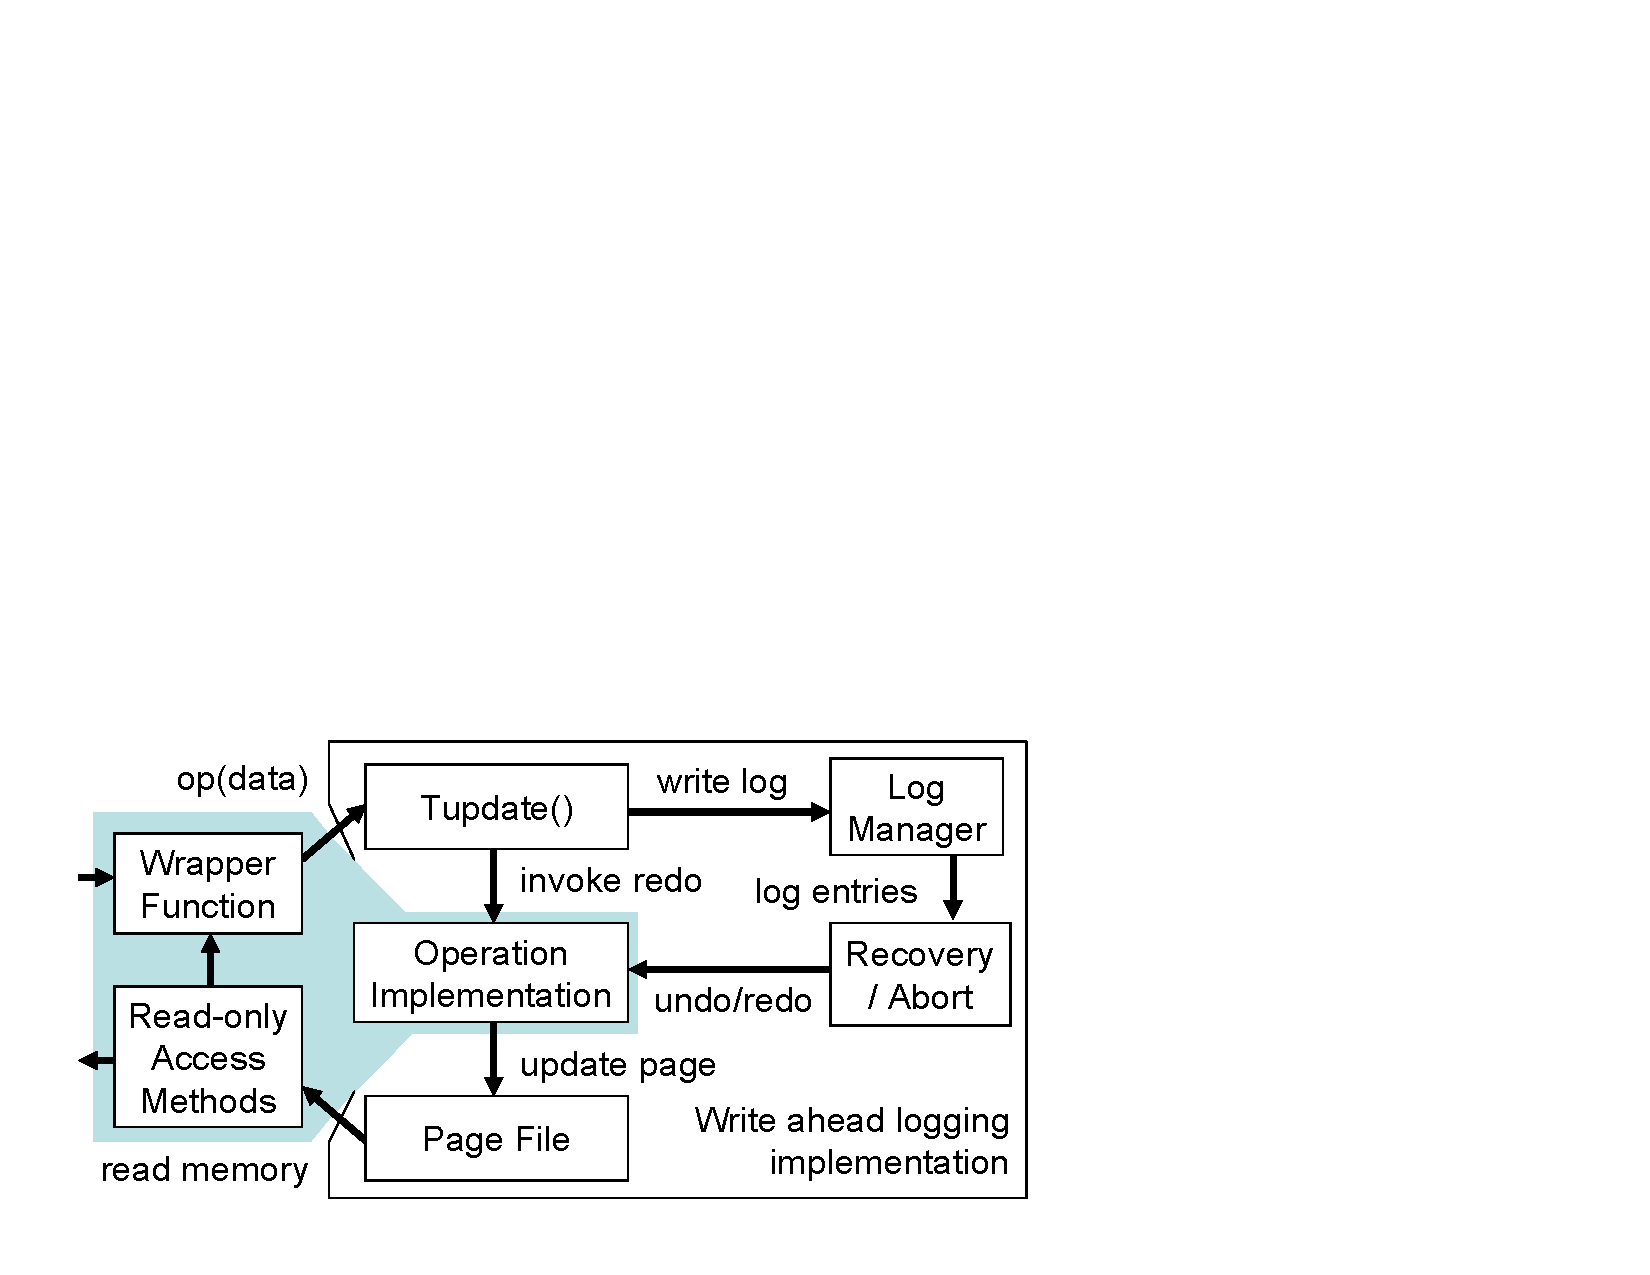
\includegraphics[%
   width=1\columnwidth]{figs/structure.pdf}
\caption{\sf\label{fig:structure} The portions of \yad that new operations interact with directly.}
\end{figure}
\yad allows application developers to easily add new operations to the
system.  Many of the customizations described below can be implemented
using custom log operations.  In this section, we desribe how to add a
``typical'' Steal/no-Force operation that supports concurrent
transactions, full physiological logging, and per-page LSN's.  Such
opeartions are typical of high-performance commercial database
engines.

As we mentioned above, \yad operations must implement a number of
functions.  Figure~\ref{yadArch} describes the environment that
schedules and invokes these functions.  The first step in implementing
a new set of log interfaces is to decide upon interface that these log
interfaces will export to callers outside of \yad.  

These interfaces are implemented by the Wrapper Functions and Read
only access methods in Figure~\ref{yadArch}.  Wrapper functions that
modify the state of the database package any information that will be
needed for undo or redo into a data format of its choosing.  This data
structure, and an opcode associated with the type of the new
operation, are passed into Tupdate(), which copies its arguments to
the log, and then passes its arguments into the operation's REDO
function.
 
REDO modifies the page file, or takes some other action directly.  It
is essentially an iterpreter for the log entries it is associated
with.  UNDO works analagously, but is invoked when an operation must
be undone (usually due to an aborted transaction, or during recovery).
This general pattern is quite general, and applies in many cases.  In
order to implement a ``typical'' operation, the operations
implementation must obey a few more invariants:

\begin{itemize}
\item Pages should only be updated inside REDO and UNDO functions.
\item Page updates atomically update page LSN's by pinning the page.
\item If the data seen by a wrapper function must match data seen
  during REDO, then the wrapper should use a latch to protect against
  concurrent attempts to update the sensitive data (and against
  concurrent attempts to allocate log entries that update the data).
\item Nested top actions (and logical undo), or ``big locks'' (which
  reduce concurrency) should be used to implement multi-page updates.
\end{itemize}

\subsection{Linear hash table}
\begin{figure}[t]
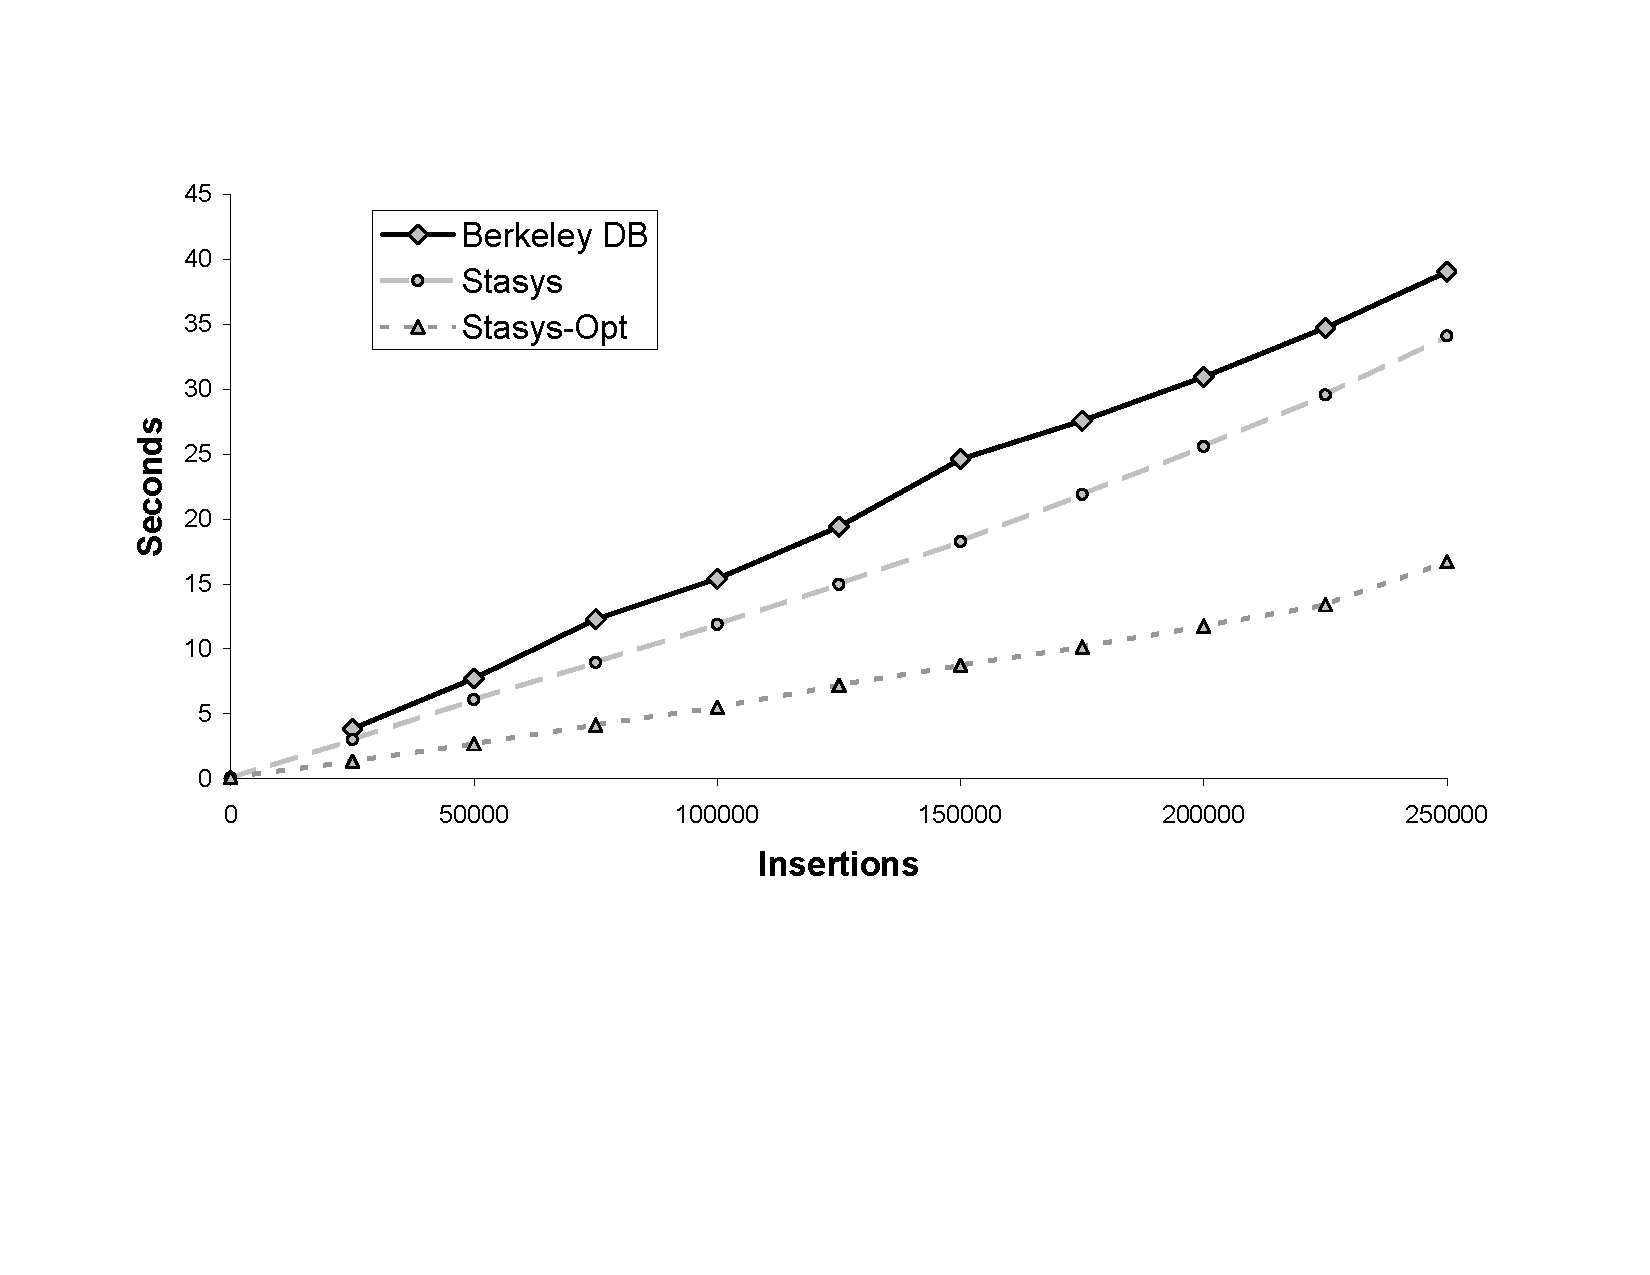
\includegraphics[%
   width=1\columnwidth]{figs/bulk-load.pdf}
%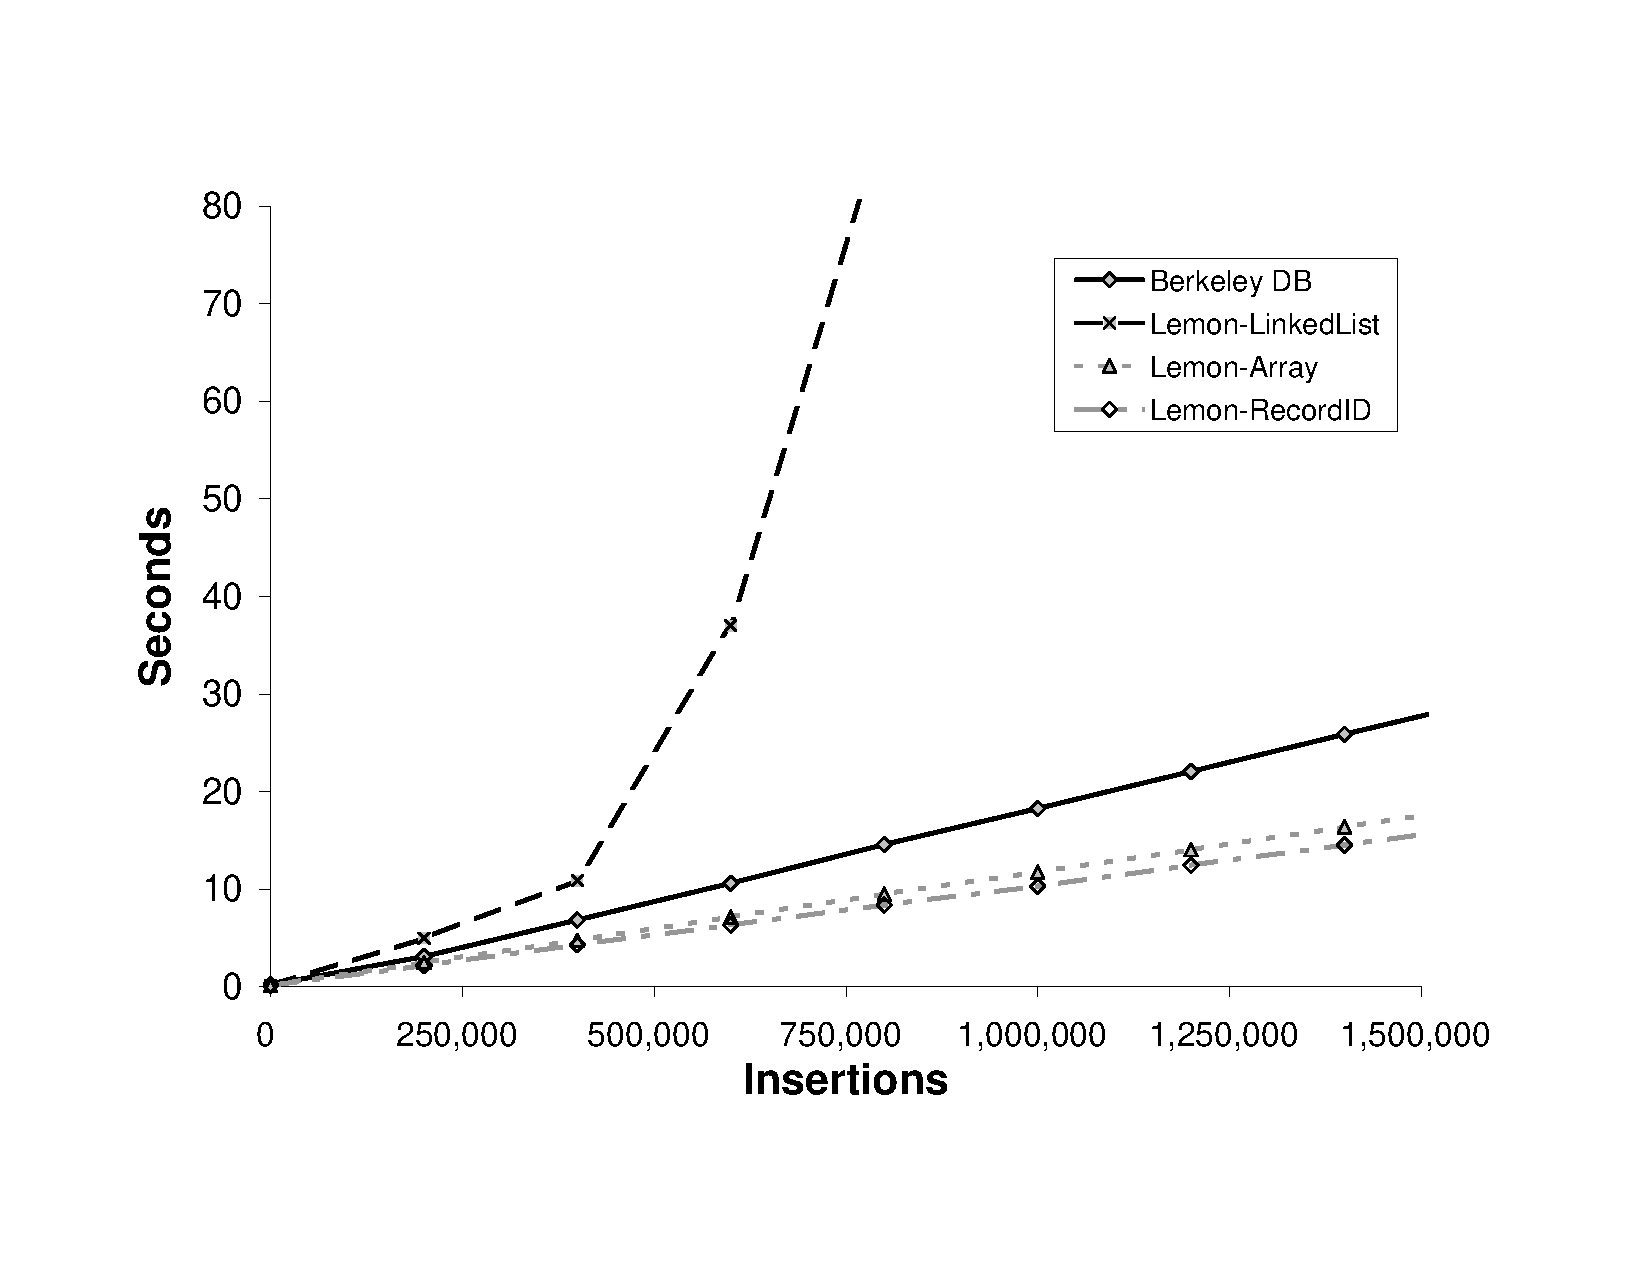
\includegraphics[%
%   width=1\columnwidth]{bulk-load-raw.pdf}
%\vspace{-30pt}
\caption{\sf\label{fig:BULK_LOAD} Performance of \yad and Berkeley DB hashtable implementations.  The
test is run as a single transaction, minimizing overheads due to synchronous log writes.}
\end{figure}
\begin{figure}[t]
%\hspace*{18pt}
%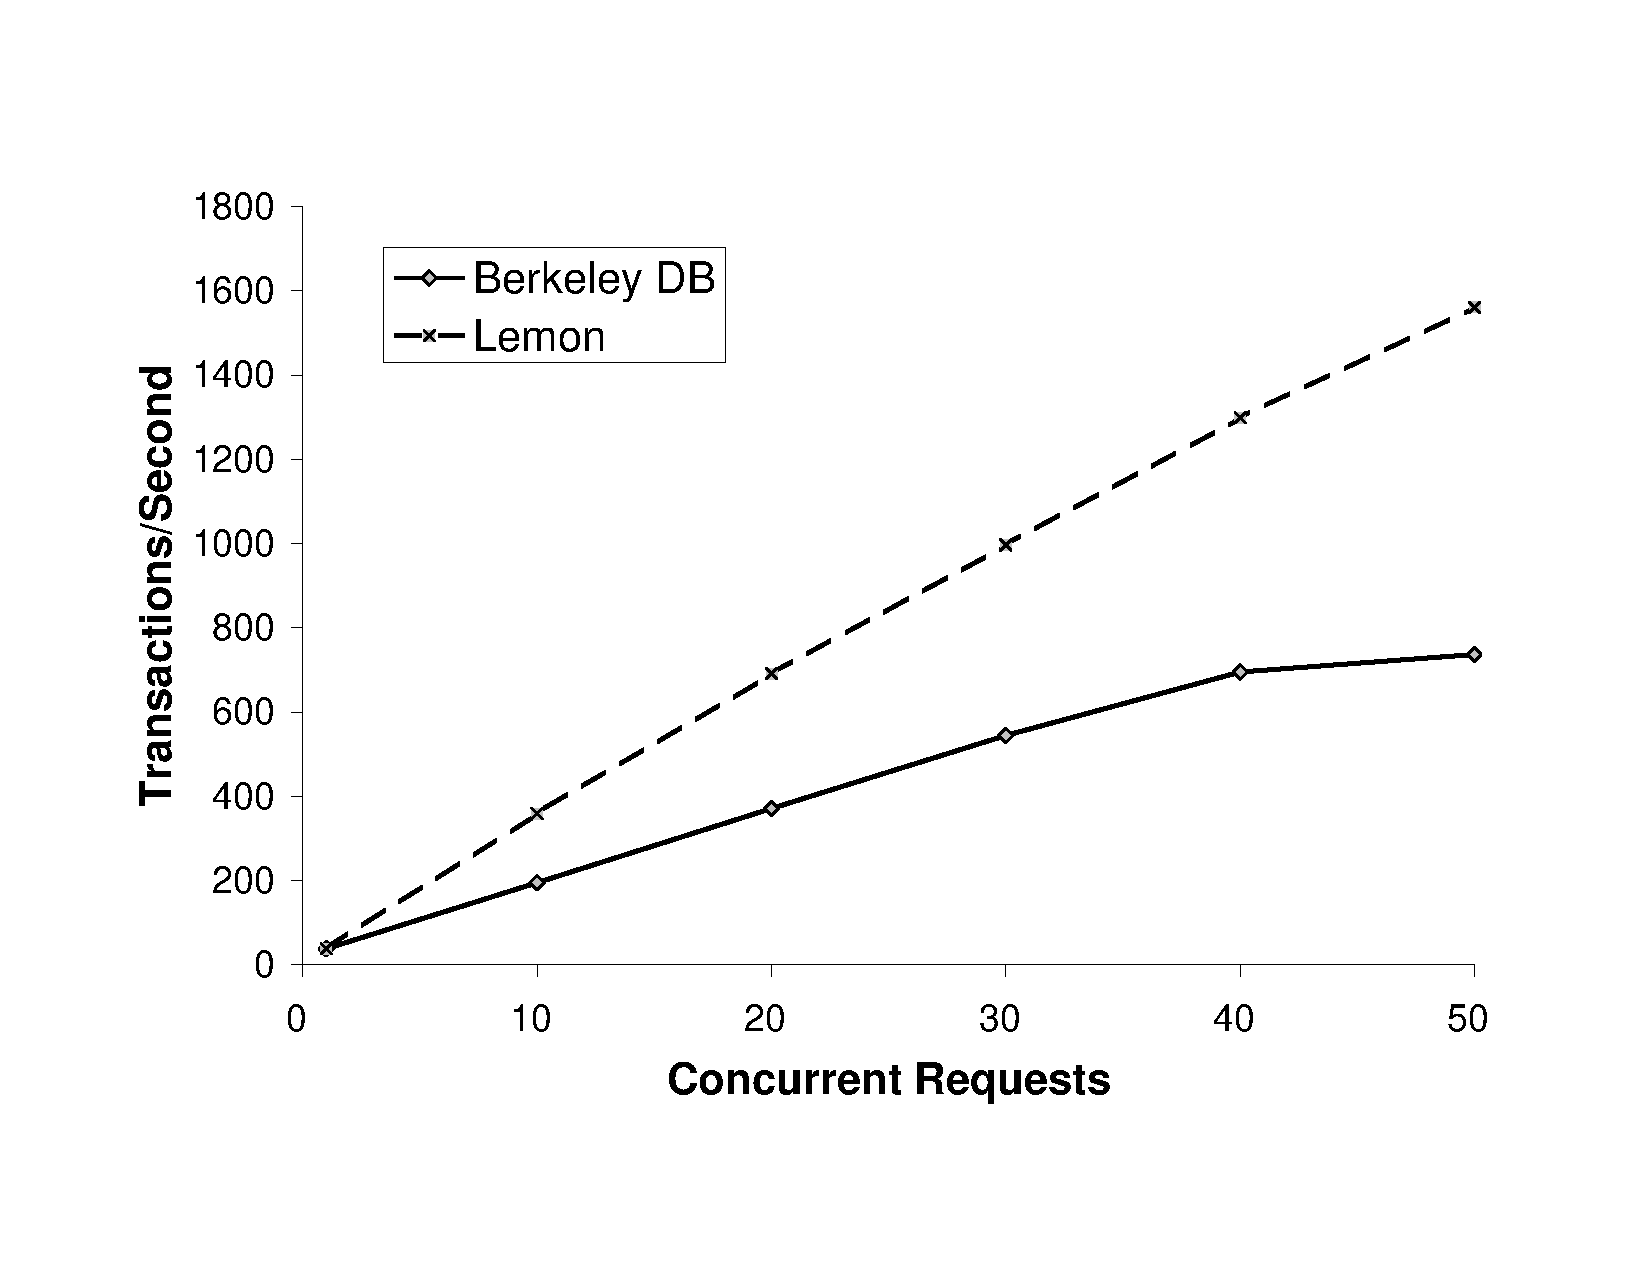
\includegraphics[%
%   width=1\columnwidth]{tps-new.pdf}
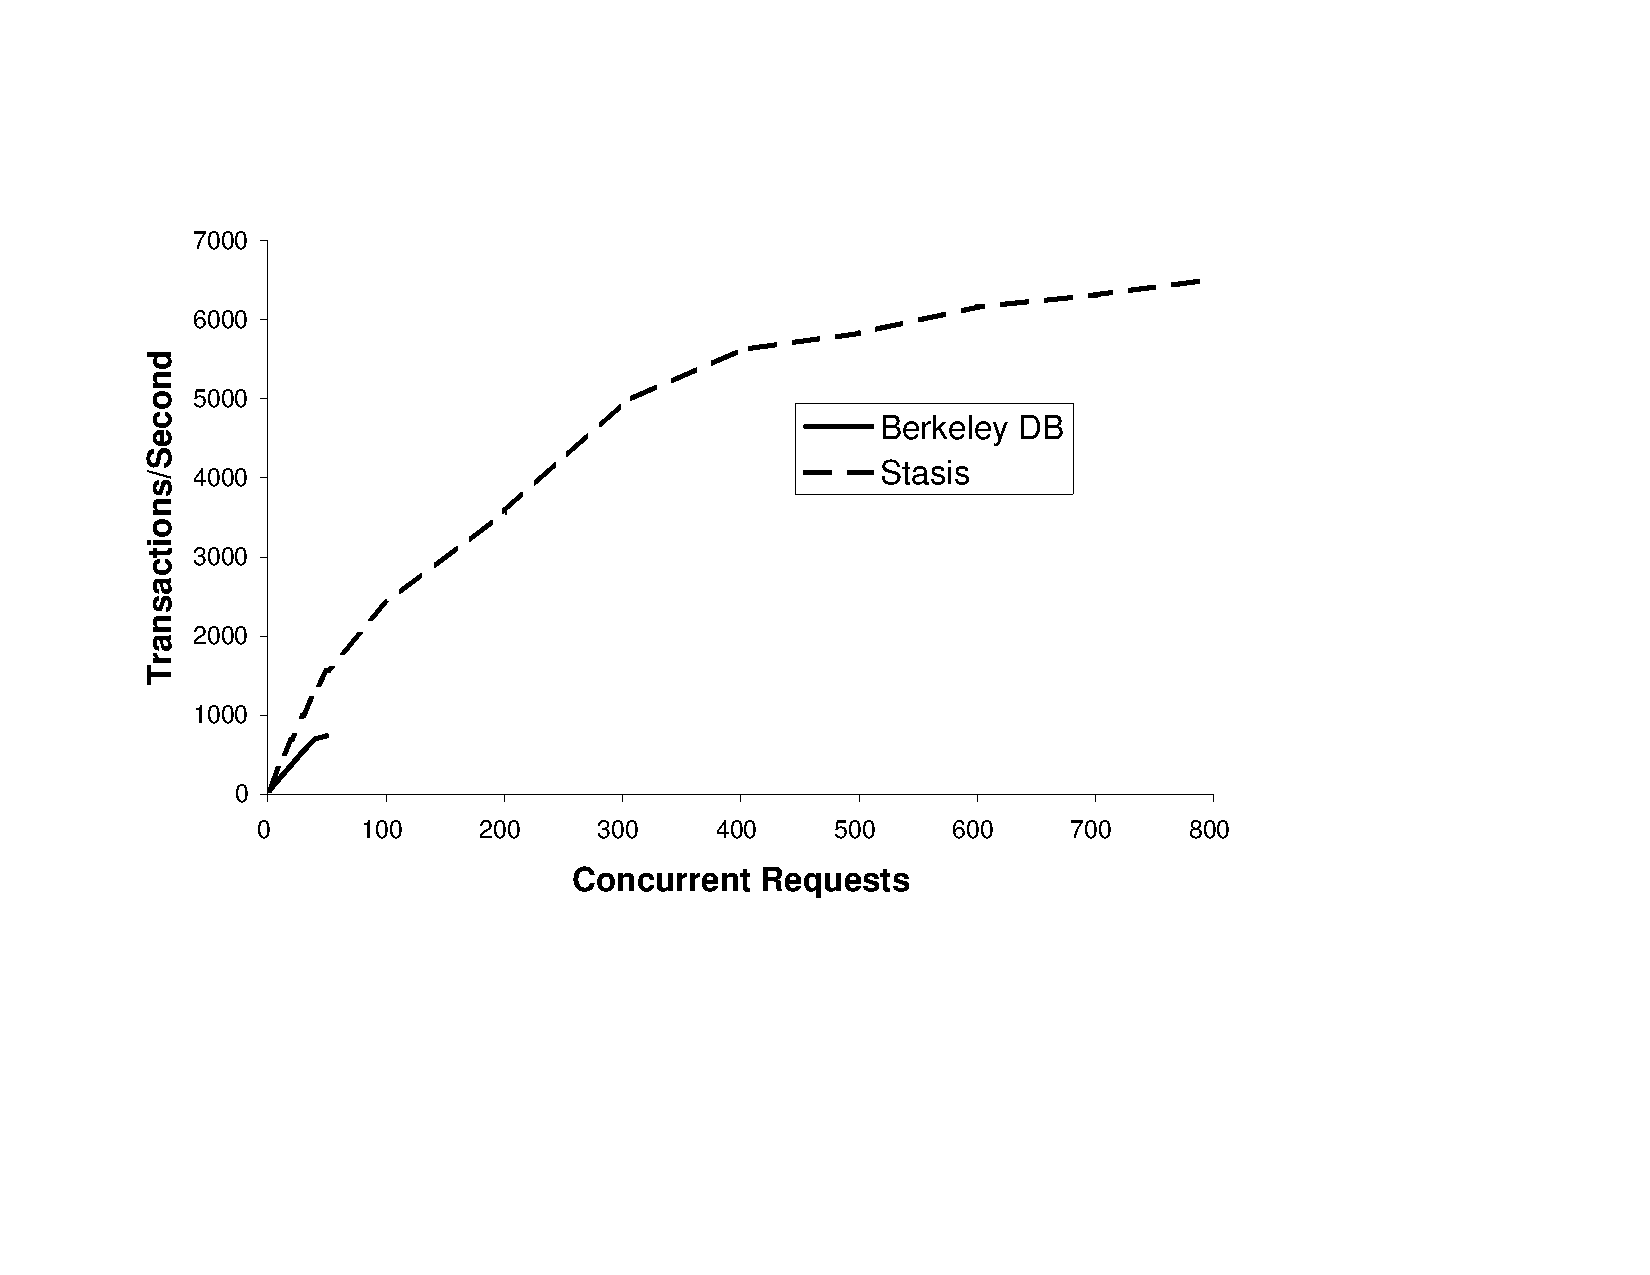
\includegraphics[%
   width=3.25in]{figs/tps-extended.pdf}
%\vspace{-36pt}
\caption{\sf\label{fig:TPS} High concurrency performance of Berkeley DB and \yad.  We were unable to get Berkeley DB to work correctly with more than 50 threads. (See text)
}
\end{figure}

Although the beginning of this paper describes the limitations of
physical database models and relational storage systems in great
detail, these systems are the basis of most common transactional
storage routines.  Therefore, we implement key-based storage, and a
primititve form of linksets in this section.  We argue that obtaining
obtaining reasonable performance in such a system under \yad is
straightforward, and compare a simple hash table to a hand-tuned (not
straightforward) hash table, and Berkeley DB's implementation.

The simple hash table uses nested top actions to atomically update its
internal structure.  It is based on a linear hash function, allowing
it to incrementally grow its buffer list.  It is based on a number of
modular subcomponents, notably a growable array of fixed length
entries, and the user's choice of two different linked list
implementations.  The hand-tuned hashtable also uses a {\em linear} hash
function,~\cite{lht} but is monolithic, and uses carefully ordered writes to
reduce log bandwidth, and other runtime overhead.  Berkeley DB's
hashtable is a popular, commonly deployed implementation, and serves
as a baseline for our experiements.

Both of our hashtables outperform Berkeley DB on a workload that
bulkloads the tables by repeatedly inserting key, value pairs into
them.  We do not claim that our partial implementation of \yad
generally outperforms Berkeley DB, or that it is a robust alternative
to Berkeley DB.  Instead, this test shows that \yad is comparable to
existing systems, and that its modular design does not introduce gross
inefficiencies at runtime.

The comparison between our two hash implementations is more
enlightening.  The performance of the simple hash table shows that
quick, straightfoward datastructure implementations composed from
simpler structures behave reasonably well in \yad.  The hand-tuned
implementation shows that \yad allows application developers to
optimize the primitives they build their applications upon.  In the
best case, past systems allowed application developers to providing
hints to improve performance.  In the worst case, a developer would be
forced to redesign the application to avoid sub-optimal properties of
the transactional data structure implementation.

Figure~\ref{lhtThread} describes performance of the two systems under
highly concurrent workloads.  For this test, we used the simple
(unoptimized) hash table, since we are interested in the performance a
clean, modular data structure that a typical system implementor would
be likely to produce, not the performance of our own highly tuned,
monolithic, implementations.

Both Berekely DB and \yad can service concurrent calls to commit with
a single synchronous I/O.\endnote{The multi-threaded benchmarks
  presented here were performed using an ext3 filesystem, as high
  concurrency caused both Berkeley DB and \yad to behave unpredictably
  when reiserfs was used.  However, \yad's multi-threaded throughput
  was significantly better that Berkeley DB's under both systems.}
\yad scaled quite well, delivering over 6000 transactions per
second,\endnote{This test was run without lock managers, so the
  transactions obeyed the A, C, and D properties.  Since each
  transaction performed exactly one hashtable write and no reads, they
  obeyed I (isolation) in a trivial sense.}  and provided roughly
double Berkeley DB's throughput (up to 50 threads).  We do not report
the data here, but we implemented a simple load generator that makes
use of a fixed pool of threads with a fixed think time.  We found that
the latency of Berkeley DB and \yad were similar, addressing concerns
that \yad simply trades latency for throughput during the concurrency
benchmark.

\subsection{Object serialization}

\begin{figure*}[t!]
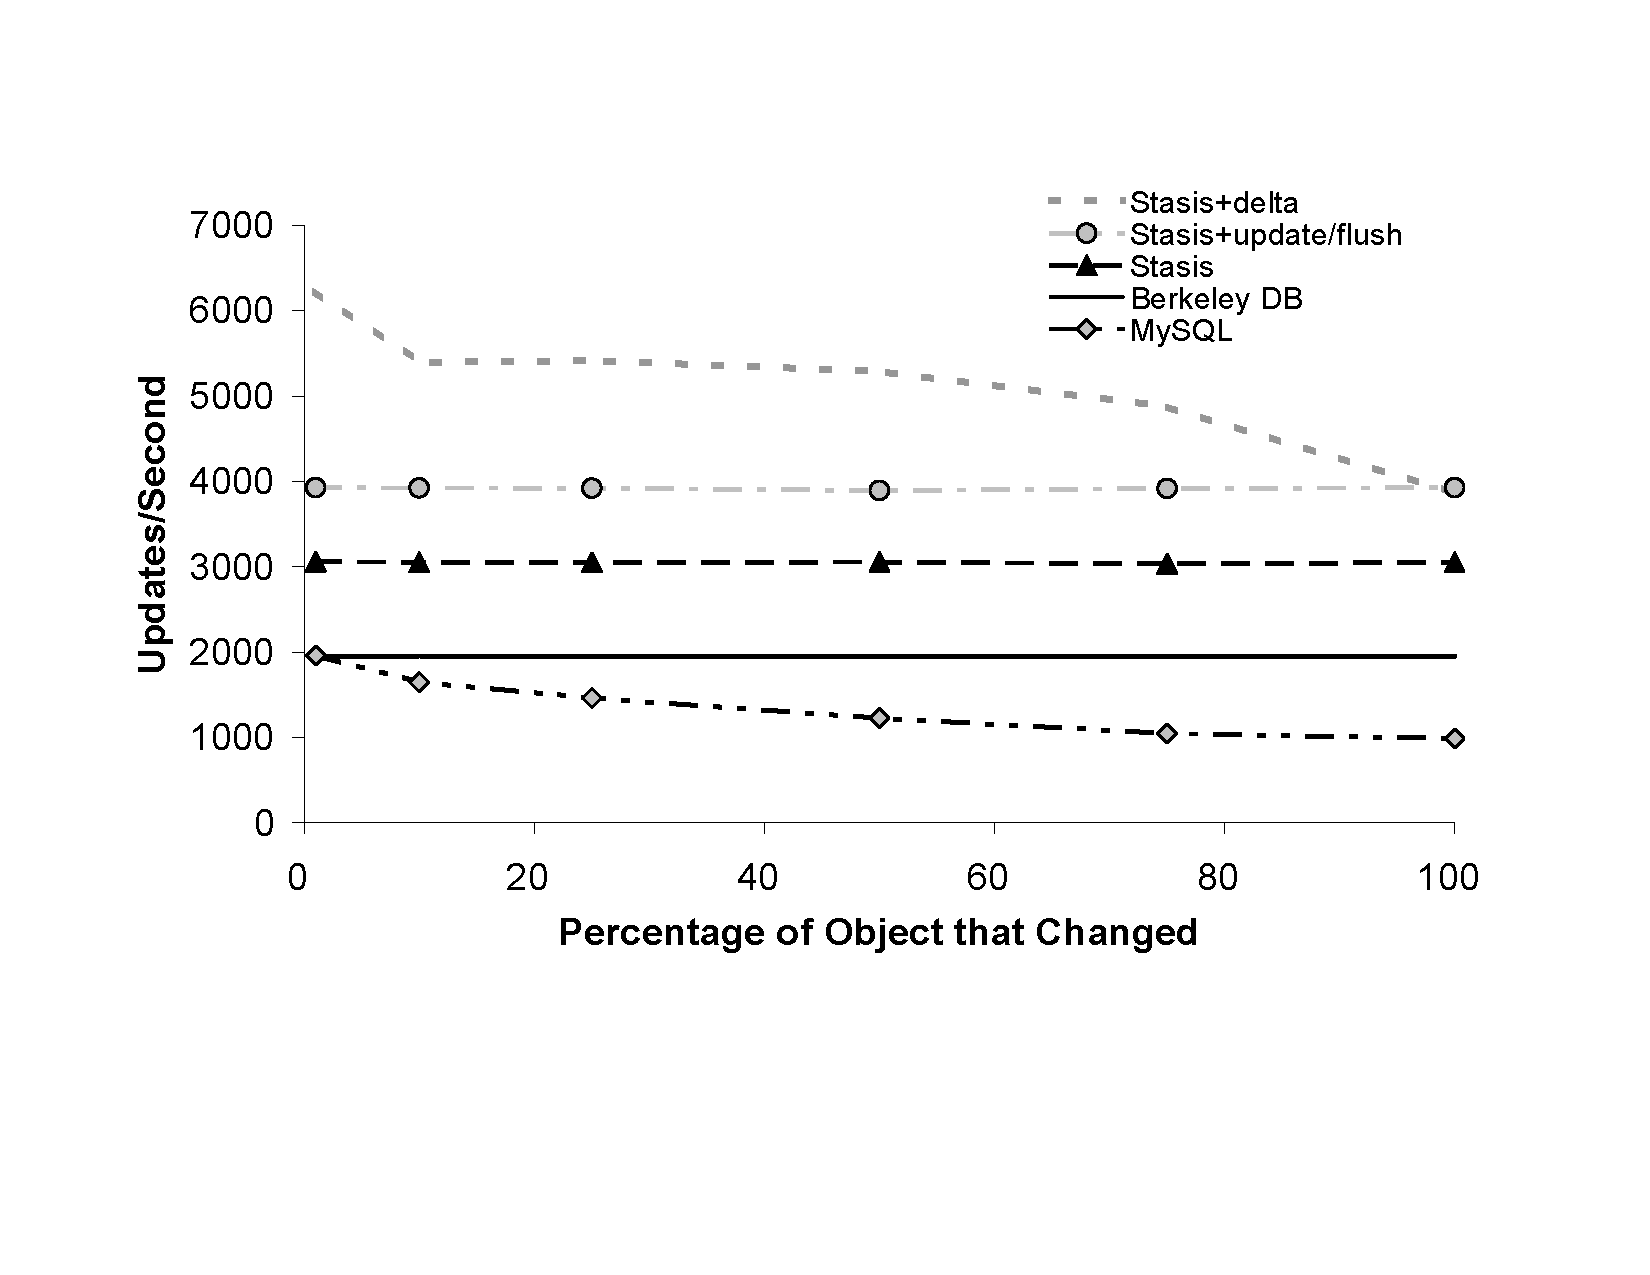
\includegraphics[width=3.3in]{figs/object-diff.pdf}
\hspace{.3in}
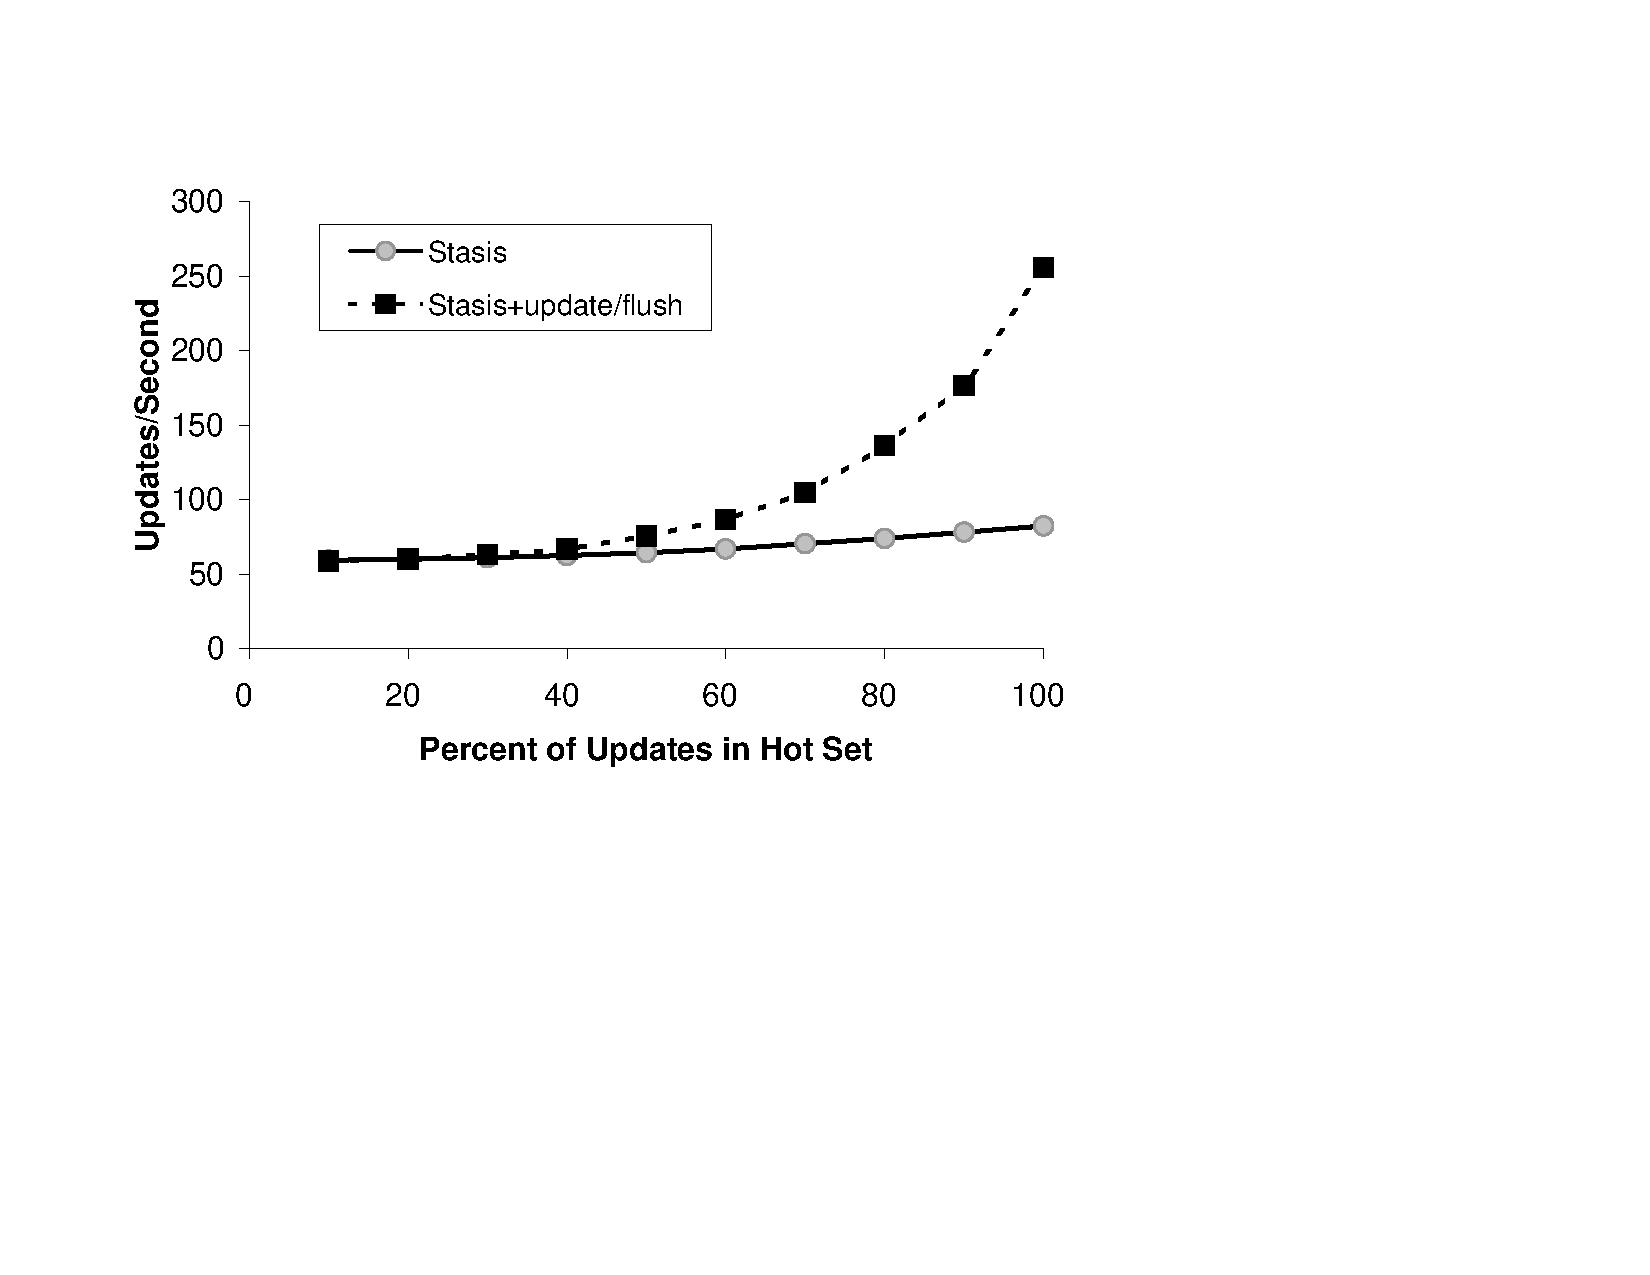
\includegraphics[width=3.3in]{figs/mem-pressure.pdf}
\vspace{-.15in}
\caption{\sf \label{fig:OASYS}
The effect of \yad object serialization optimizations under low and high memory pressure.}
\end{figure*}

\subsection{Object persistance mechanisms}
\rcs{ This belongs somewhere else: Instead, it leaves decisions regarding abstract data types and
algorithm design to system developers or language designers.  For
instance, while \yad has no concept of object oriented data types, two
radically different approaches toward object persistance have been
implemented on top of it~\ref{oasys}.}

\rcs{We could have just as easily written a persistance mechanism for a
functional programming language, or a particular application (such as
an email server).  Our experience building data manipulation routines
on top of application-specific primitives was favorable compared to
past experiences attempting to restructure entire applications to
match pre-existing computational models, such as SQL's declarative
interface.}




Numerous schemes are used for object serialization.  Support for two
different styles of object serialization have been eimplemented in
\yad.  The first, pobj, provided transactional updates to objects in
Titanium, a Java variant.  It transparently loaded and persisted
entire graphs of objects.

The second variant was built on top of a generic C++ object
serialization library, \oasys.  \oasys makes use of pluggable storage
modules to actually implement persistant storage, and includes plugins
for Berkeley DB and MySQL.  This section will describe how the \yad's
\oasys plugin reduces the runtime serialization/deserialization cpu
overhead of write intensive workloads, while using half as much system
memory as the other two systems.

We present three variants of \yad here.  The first treats \yad like
Berkeley DB.  The second customizes the behavior of the buffer
manager.  Instead of maintaining an up-to-date version of each object
in the buffer manager or page file, it allows the buffer manager's
view of live application objects to become stale.  This is safe since
the system is always able to reconstruct the appropriate page entry
form the live copy of the object.

The reason it would be difficult to do this with Berkeley DB is that
we still need to generate log entries as the object is being updated.
Otherwise, commit would not be durable, and the application would be
unable to abort() transactions.  Even if we decided to disallow
application aborts, we would still need to write log entries
committing.  This would cause Berekley DB to write data back to the
page file, increasing the working set of the program, and increasing
disk activity.

Under \yad, we implemented this optimization by adding two new
operations, update(), which only updates the log, and flush(), which
updates the page file.  We decrease the size of the page file, so
flush() is likely to incur disk overhead.  However, we have roughly
doubled the number of objects that are cached in memory, and expect
flush() to be called relatively infrequently.

The third \yad plugin to \oasys incorporated all of the updates of the
second, but arranged to only the changed portions of objects to the
log.

Figure~\ref{objectSerialization} presents the performance of the three
\yad optimizations, and the \oasys plugins implemented on top of other
systems.  As we can see, \yad performs better than the baseline
systems.  More interestingly, in non-memory bound systems, the
optimizations nearly double \yad's performance, and we see that in the
memory-bound setup, update/flush indeed improves memory utilization.


\subsection{Manipulation of logical log entries}

\begin{figure}
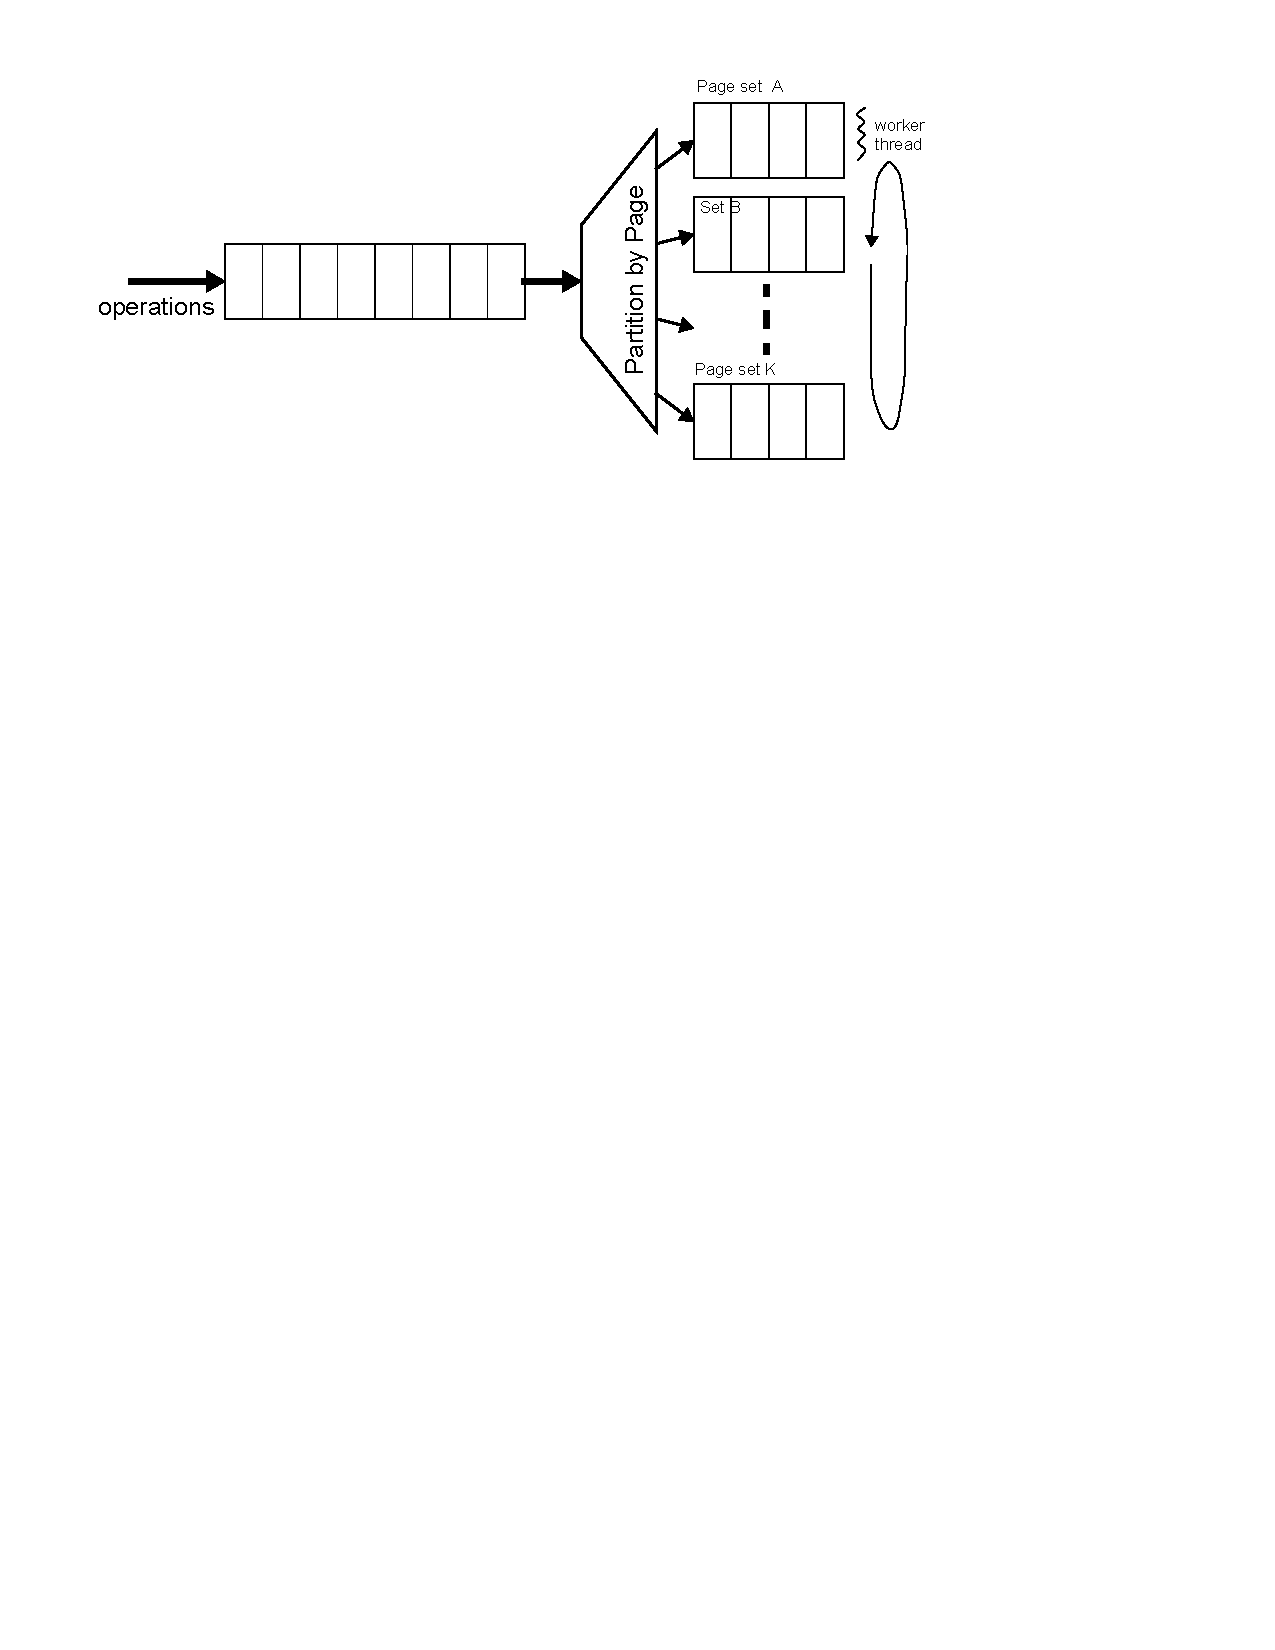
\includegraphics[width=1\columnwidth]{figs/graph-traversal.pdf}
\vspace{-24pt}
\caption{\sf\label{fig:multiplexor} Because pages are independent, we
can reorder requests among different pages. Using a log demultiplexer,
we partition requests into independent queues, which can be 
handled in any order, improving locality and merging opportunities.}
\end{figure}
\begin{figure}[t]
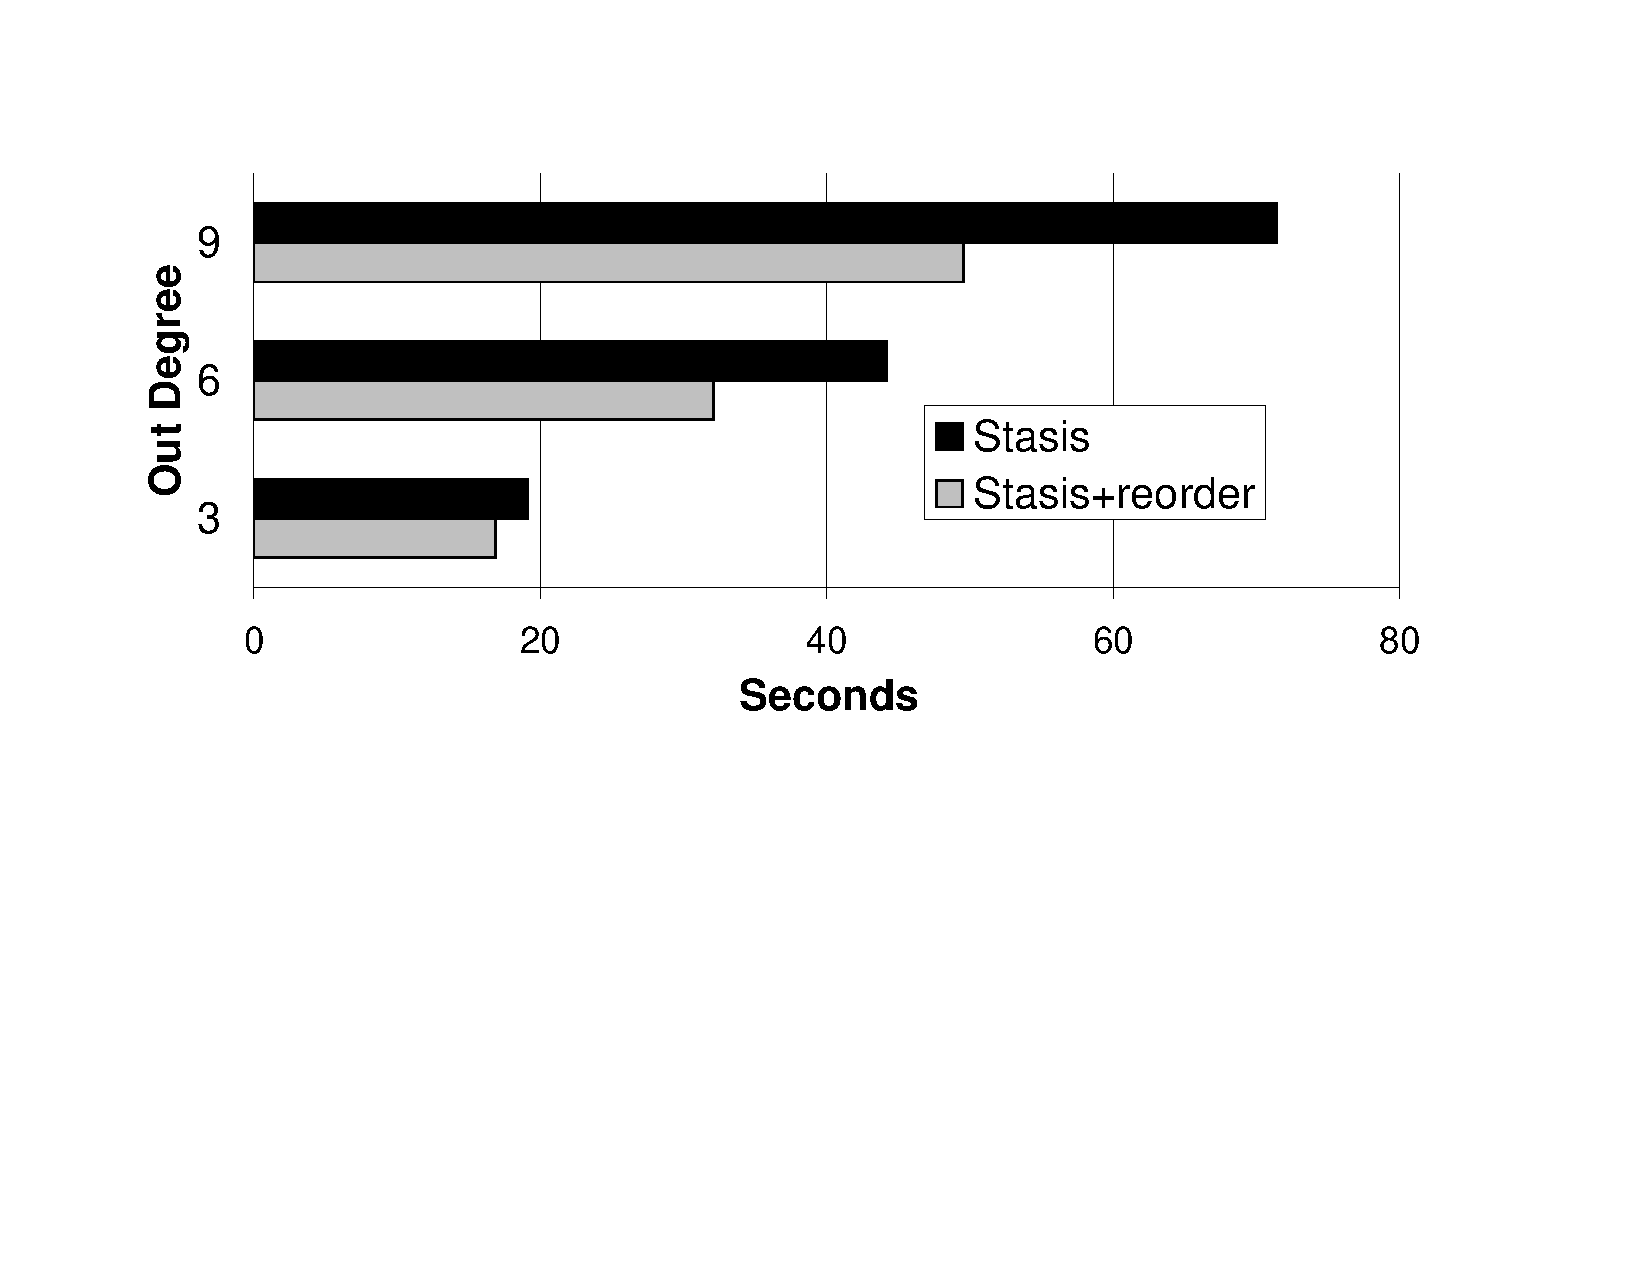
\includegraphics[width=3.3in]{figs/oo7.pdf}
\vspace{-15pt}
\caption{\sf\label{fig:oo7} oo7 benchmark style graph traversal.  The optimization performs well due to the presence of non-local nodes.}
\end{figure}

\begin{figure}[t]
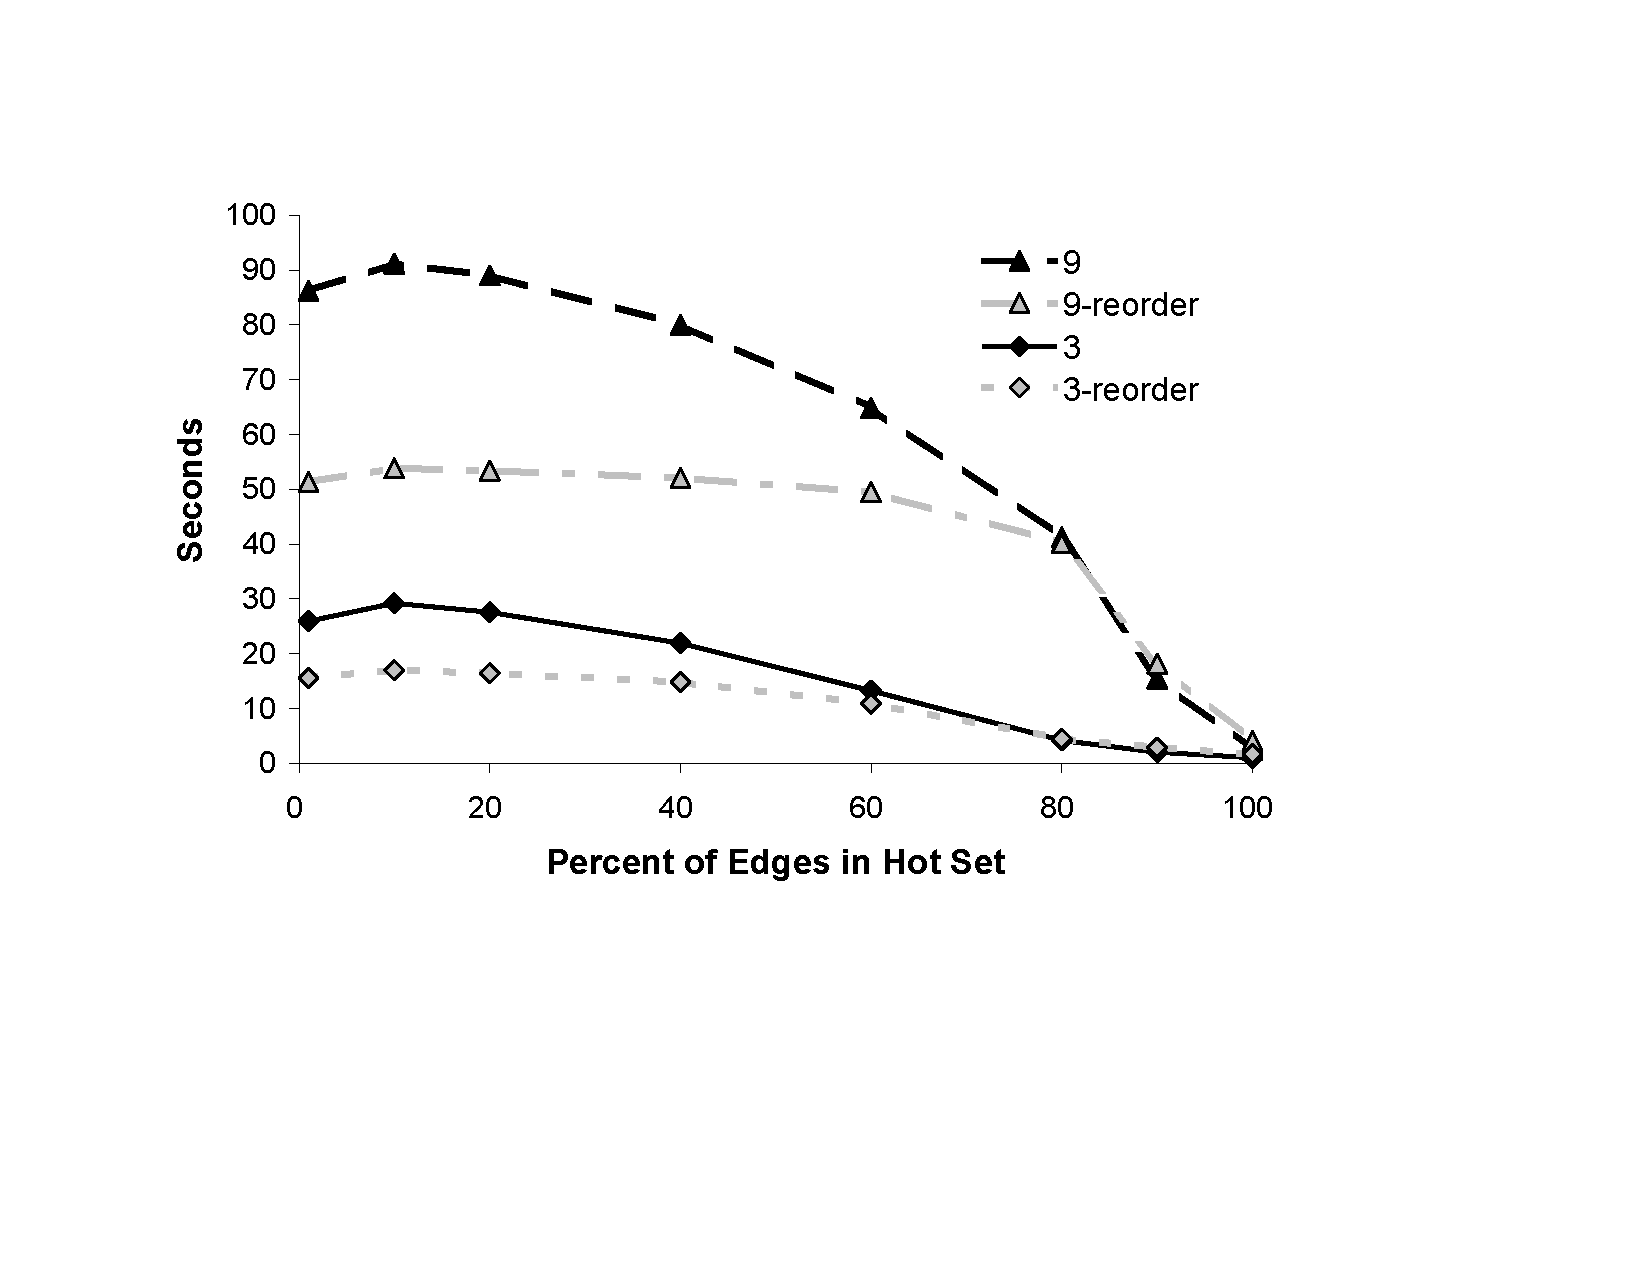
\includegraphics[width=3.3in]{figs/trans-closure-hotset.pdf}
\vspace{-12pt}
\caption{\sf\label{fig:hotGraph} Hot set based graph traversal for random graphs with out-degrees of 3 and 9.  Here
we see that the multiplexer helps when the graph has poor locality.
However, in the cases where depth first search performs well, the
reordering is inexpensive.}
\end{figure}

Database optimizers operate over relational algebra expressions that
will correspond to sequence of logical operations at runtime.  \yad
does not support query languages, relational algebra, or other general
purpose primitves.

However, it does include an extendible logging infrastructure, and any
operations that make user of physiological logging implicitly
implement UNDO (and often REDO) functions that interpret logical
operations.

Logical operations often have some nice properties that this section
will exploit.  Because they can be invoked at arbitrary times in the
future, they tend to be independent of the database's physical state.
They tend to be inverses of operations that programmer's understand.
If each method in the API exposed to the programmer is the inverse of
some other method in the API, then each logical operation corresponds
to a method the programmer can manually invoke.

Because of this, application developers can easily determine whether
logical operations may safely be reordered, transformed, or even
dropped from the stream of requests that \yad is processing.  Even
better, if requests can be partitioned in a natural way, load
balancing can be implemented by spliting requests across many nodes.
Similarly, a node can easily service streams of requests from multiple
nodes by combining them into a single log, and processing the log
using operaiton implementations.  Furthermore, application-specific
procedures that are analagous to standard relational algebra methods
(join, project and select) could be used to efficiently transform the data
before it reaches the page file, while it is layed out sequentially
in memory.

Note that read-only operations do not necessarily generate log
entries.  Therefore, applications may need to implement custom
operations to make use of the ideas in this section.

Although \yad has rudimentary support for a two-phase commit based
cluster hash table, we have not yet implemented a logical log based
networking primitives.  Therefore, we implemented some of these ideas
in a single node configuration in order to increase request locality
during the traversal of a random graph.  The graph traversal system
takes a sequence of (read) requests, and partitions them using some
function.  It then proceses each partition in isolation from the
others.  We considered two partitioning functions.  The first, which
is really only of interested in the distributed case, partitions the
requests according to the hash of the node id they refer to.  This
would allow us to balance the graph traversal across many nodes.  (We
expect the early phases of such a traversal to be bandwidth, not
latency limited, as each node would stream large sequences of
asynchronous requests to the other nodes.) 

The second partitioning function, which was used to produce
Figure~\ref{hotset} partitions requests by their position in the page
file.  When the graph has good locality, a normal depth first search
traversal and the prioritized traversal perform well.  As locality
decreases, the partitioned traversal algorithm's performance degrades
less than the naive traversal.

**TODO This really needs more experimental setup... look at older draft!**

\subsection{LSN-Free pages}

In Section~\ref{todo}, we describe how operations can avoid recording
LSN's on the pages they modify.  Essentially, opeartions that make use
of purely physical logging need not heed page boundaries, as
physiological operations must.  Recall that purely physical logging
interacts poorly with concurrent transactions that modify the same
data structures or pages, so LSN-Free pages are not applicable in all
situations.

Consider the retreival of a large (page spanning) object stored on
pages that contain LSN's.  The object's data will not be contiguous.
Therefore, in order to retrive the object, the transaction system must
load the pages contained on disk into memory, allocate buffer space to
allow the object to be read, and perform a byte-by-byte copy of the
portions of the pages that contain the large object's data.  Compare
this approach to a modern filesystem, which allows applications to
perform a DMA copy of the data into memory, avoiding the expensive
byte-by-byte copy of the data, and allowing the CPU to be used for
more productive purposes.  Furthermore, modern operating systems allow
network services to use DMA and ethernet adaptor hardware to read data
from disk, and send it over a network socket without passing it
through the CPU.  Again, this frees the CPU, allowing it to perform
other tasks.

We beleive that LSN free pages will allow reads to make use of such
optimizations in a straightforward fashion.  Zero copy writes could be
performed by performing a DMA write to a portion of the log file.
However, doing this complicates log truncation, and does not address
the problem of updating the page file.  We suspect that contributions
from the log based filesystem literature can address these problems in
a straightforward fashion.

Finally, RVM, recoverable virtual memory, made use of LSN-free pages
so that it could use mmap() to map portions of the page file into
application memory.  However, without support for logical log entries
and nested top actions, it would be difficult to implement a
concurrent, durable data structure using RVM.  We plan to add RVM
style transactional memory to \yad in a way that is compatible with
fully concurrent collections such as hash tables and tree structures.

\section{Conclusion}

\section{Acknowledgements}

\section{Availability}

Additional information, and \yad's source code is available at:

\begin{center}
{\tt http://\yad.sourceforge.net/}
\end{center}

{\footnotesize \bibliographystyle{acm}
\nocite{*}
\bibliography{LLADD}}

\theendnotes

\end{document}







